\documentclass[12pt, a4paper]{article}
\usepackage{enumitem}
\setlist[enumerate]{label = (\roman*)}
\usepackage{amsmath}
\usepackage{mathtools}
\usepackage{amssymb}
\usepackage{amsthm}
\theoremstyle{definition}
\newtheorem{example}{Example}

\usepackage{tikz}
\usepackage{hyperref}

\newcommand{\summation}[2]{\sum\limits_{#1}^{#2}}
\newcommand{\limit}[2]{\lim\limits_{#1\to #2}}
\newcommand{\vep}{\varepsilon}
\newcommand{\union}[2]{\cup_{#1}^{#2}}
\newcommand{\m}[1]{\mathcal{#1}}
\newcommand{\minus}{\textbackslash}
\newcommand{\intersection}[2]{\cup_{#1}^{#2}}

\begin{document}
\begin{example}[Empty $\max_{\succsim}$]
Consider $X=\mathbb{R}$ and $\succsim$ is more is better and $Y=(0,1)$.
\[
\max_{\succsim}\,Y=\emptyset.
\]
\end{example}

\begin{example}[Transitivity, quasi-transitivity, Acyclicity]
We give two examples. First example satisfies quasi-transitivity but fails to transitivity, second example satisfies acyclicity but fails to quasi-transitivity.
\begin{enumerate}
\item consider $X=\mathbb{R}$ and $\succsim_1$ such that for $x,y\in\mathbb{R}$, $x\succsim_1 y\iff x\geq y+1$. $\succsim_1$ satisfies quasi-transitivity but not transitive;
\item consider $X=\{x_1,x_2,x_3\}$ and $\succsim_2=\{(x_1,x_2),(x_2,x_3)\}$.
\end{enumerate}
\end{example}

\begin{example}[Some remark]
Notice that for acyclicity, ``not $x_n\succ x_1$" does not imply that $x_1\succsim x_n$, the reason is $\succsim$ may not be complete.
\end{example}

\begin{example}[Satisfying contraction but violating expansion]
Let $X=\{a,b,c\}$ and consider the following choice function.
\begin{center}
\begin{tabular}{c c}
$Y$ & $C(Y)$ \\
\hline
$ab$ & $ab$ \\
$bc$ & $bc$ \\
$ac$ & $ac$ \\
$abc$ & $a$ \\
\end{tabular}
\end{center}
This choice function violates expansion, because $b\in C(\{a,b\})$ and $b\in C(\{b,c\})$, however $b\notin C(\{a,b,c\})$.
\end{example}

\begin{example}[Satisfying strong expansion but violating contraction]
Let $X=\{a,b,c\}$ and consider the following choice function.
\begin{center}
\begin{tabular}{c c}
$Y$ & $C(Y)$ \\
\hline
$ab$ & $a$ \\
$bc$ & $b$ \\
$ac$ & $c$ \\
$abc$ & $abc$ \\
\end{tabular}
\end{center}
This choice function violates contraction, because $a\in C(\{a,b,c\})$ however, $a\notin C(\{a,c\})$.
\end{example}

\begin{example}
The notion of WARP is equivalent to the following condition: for all $Y,Z\in\mathcal{M}(X)$ and $x,y\in Y\cap Z$,
\[
x\in C(Y)\text{ and }y\in C(Z)\text{ implies }x\in C(Z).
\]
\begin{proof}
Proof breaks into two parts.
\begin{enumerate}[label = (\roman*)]
\item ``$\rightarrow$": as $(Y\cap Z)\subset Y$ and $\{x\}\subset \big(C(Y)\cap (Y\cap Z)\big)$, hence WARP implies $C(Y\cap Z) = C(Y)\cap (Y\cap Z)$. We can conclude: $x\in C(Y\cap Z)$. Applying $Y\cap Z$ and $Z$ with WARP, we finally get: $C(Y\cap Z)=C(Z)\cap (Y\cup Z)$. Hence, $x\in C(Z)$.
\item ``$\leftarrow$": let $Z\subset Y$ and $C(Y)\cap Z\neq \emptyset$. 
\begin{enumerate}
\item $\forall x\in C(Z)$, we have: $x\in Z=Z\cap Y$, therefore $x\in C(Y)$, which implies $C(Z)\subset C(Y)\cap Z$;
\item $\forall x\in C(Y)\cap Z$, we have: $x\in Z\cap Y$ and $x\in C(Y)$, therefore $x\in C(Z)$, which implies $C(Y)\cap Z \subset C(Z)$.
\end{enumerate}
Therefore, $C(Y)\cap Z = C(Z)$.
\end{enumerate}
\end{proof}
\end{example}

\begin{example}[Rationalizable but not by quasi-transitive relation]
We construct a relation that is rationalizable but not by a quasi-transitive relation.
\begin{center}
\begin{tabular}{c c}
$Y$ & $C(Y)$ \\
\hline
$ab$ & $b$ \\
$ac$ & $ac$ \\
$bc$ & $c$ \\
$abc$ & $c$ \\
\end{tabular}
\end{center}
Therefore, $b\succ_Ca$ and $a\sim_Cc$ and $c\succ_Cb$, which clearly violates quasi-transitivity. 
\end{example}

\begin{example}[Some observations]
We have the following two observations.
\begin{enumerate}[label = (\roman*)]
\item every preference is semi-order;
\item semi-order is quasi-transitive, however not every quasi-transitive relation is semi-order.
\end{enumerate}
Following two examples illustrating the converse of observations above.
\begin{enumerate}[label = (\roman*)]
\item not every semi-order is preference. Consider $X=\{x,y,z\}$ and $x\sim y\sim z$ and $x\succ z$. It's semi-order but not a preference.
\item not every quasi-transitive preference is semi-order. Consider $X=\{x,y,z,w\}$ with $x\succ y$ and $z\succ w$ and indifference otherwise. Clearly, it's quasi-transitive but not semi-order.
\end{enumerate}
\end{example}

\begin{example}[Independence of vNM3]
lexicographic preferences. Let $A=\{a_1,a_2,\dots,a_n\}$ and define $\succsim$ on $\m{L}(A)$ as following:
\begin{enumerate}
\item $p\sim p$ for all $p\in\m{L}(A)$;
\item $p\succ q$ if and only if there exists $k\in[n]$ so that $p(a_i) = q(a_i)$ for all $i<k$ and $p(a_k)>q(a_k)$.
\end{enumerate}
Consider the following three lotteries: $p_1 = (\frac{2}{3},\frac{1}{6},\dots)\succ p_2 = (\frac{1}{3},\frac{1}{2},\dots)\succ p_3 = (\frac{1}{3},\frac{1}{3},\dots)$. However any convex combination of $p_1$ and $p_3$ is strictly preferred to $p_2$.
\end{example}

\begin{example}[Independence of F3]
We present an example violating De Finetti's axiom $3$ but remaining satisfying other axioms. Let $S=\{s_1,\dots,s_n\}$ for some $n\in \mathcal{N}$. Define $\succsim$ by letting, $f\sim g$ if and only if $f=g$ and $f\succ g$ if and only if there is a $k\in[n]$ such that $f(s_i)=g(s_i)$ for all $i<k$ and $f(s_k)>g(s_k)$. Let's consider for the case when $n=2$ and $f=(1,1)$. Then, $U_{\succsim}(f) = \{(x,y):x>1\text{ or }x=1,y\geq 1\}$ which is not open.

\begin{figure}[h!]
\centering
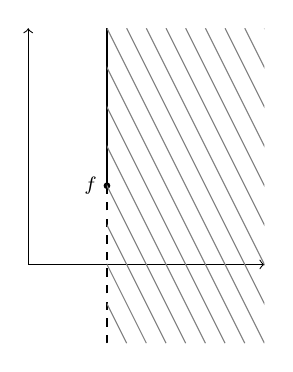
\begin{tikzpicture}[font = \scriptsize]
\draw [<->] (0,3) -- (0,0) -- (3,0);
\draw [fill = black] (1,1) circle (1pt); 
\draw [dashed] (1,-1) -- (1,3);
\draw (1,1) -- (1,3);
\node [left] at (1,1) {$f$};
\clip (1,3) -- (3,3) -- (3,-1) -- (1,-1) -- (1,3);
\foreach \x in {-3,-2,-1.75,-1.5,-1.25,-1,-0.75,-0.5,-0.25,0,0.25,0.5,0.75,1,1.25,1.5,1.75,2,2.25,2.5,2.75}
\draw [xshift = \x cm, thin, gray] (1,3) -- (3,-1);
\end{tikzpicture}
\caption{$U_{\succsim}(f)$}
\end{figure}
\end{example}




























\end{document}